\chapter{Глава 4}\label{ch:ch4}

\section{Устройство относительного измерения момента}\label{sec:ch4/sect1}


В филиале АО «Корпорация «Комета» – «НПЦ ОЭКН» создано и и аттестовано устройство относительного измерения остаточного момента (УОИОМ). На рисунке \cref{fig:yoim} представлен общий вид установки.

\begin{figure}[ht]
	\centerfloat{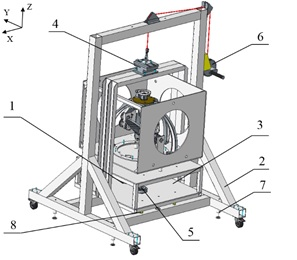
\includegraphics[scale=2]{yoiom}}
	\caption{Устройство относительного измерения остаточного момента}
	\legend{1 – маховик; 2 – платформа; 3 – измерительная платформа с изделиедержателем; 4 – зацеп настраиваемый; 5 – узел привода редукторного OZ; 6 – привод редукторный OZ;
	 7 – волконно-оптический гироскоп; 8 – конус}
	\label{fig:yoim}
\end{figure}

Стенд для измерения остаточного реактивного момента представляет собой конструкцию, обеспечивающую измеряемой аппаратуре одну степень свободы, без сухого трения. В процессе углового перемещения ОМС на основание аппаратуры действует реактивный момент. Частично этот момент компенсируется маховиками, входящими в состав ОМС. Таким образом,
стенд служит для измерения некомпенсированного внутренними средствами аппаратуры реактивного момента. Конструктивно стенд представляет собой 
крутильный маятник. Момент инерции маятника состоит из суммы моментов инерции рамы с кантователем и момента инерции аппаратуры по измеряемой оси. Кантователь входит в узел подвеса и служит для удобства 
смены измеряемой оси аппаратуры путем расположения этой оси строго вертикально по оси чувствительности подвеса. Дифференциальное уравнение колебательного звена крутильного маятника запишем  в виде [13]

\begin{samepage}
	\begin{equation}
		\label{eq:eq_yoimDiff}
		\begin{alignedat}{2}
			J\ddot{\phi}\left(t\right) + 2b\dot{\phi}\left(t\right)+c\phi\left(t\right) = M\left(t\right)
		\end{alignedat}
	\end{equation}
	\begin{align*}
		\text{где}	& \quad J - \textnormal{момент инерции;}\\           
		& \quad b - \textnormal{обобщённое вязкое трение;}        \\
		& \quad c -  \textnormal{угловая жесткость подвеса;} \\
		& \quad M(t) - \textnormal{внешний момент;}         \\
		& \quad \phi(t) -\textnormal{угол порота узла подвеса} \\
	\end{align*}
\end{samepage}

Запишем уравнение~\cref{eq:eq_yoimDiff} иначе:ъ

\begin{samepage}
	\begin{equation}
		\label{eq:eq_yoimDiff2}
		\begin{alignedat}{2}
			\phi\left(t\right)+2\xi\phi\left(t\right)+\omega_{0}^2\phi\left(t\right) = M\left(t\right)/J
		\end{alignedat}
\end{equation}
\begin{align*}
	\text{где}	& \quad \omega_0 - \textnormal{собственная частота колебательного звена;}\\           
	& \quad \xi - \textnormal{декремент затухания;}        \\
\end{align*}
\end{samepage}


На рисунке~\cref{fig:amplitude-freq-char} представлены логарифмические амплитудная и фазовая характеристики колебательного звена. Характеристики построены относительно резонансной (собственной) частоты.

\begin{figure}[ht]
	\centerfloat{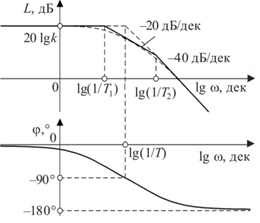
\includegraphics[scale=2]{amplitude-freq-char}}
	\caption{ЛАЧХ колебательного звена}
	\label{fig:amplitude-freq-char}
\end{figure}


Как видно из рисунка, колебательное звено не искажает входного сигнала ни по амплитуде вплоть до области, близкой к собственной частоте колебаний. В области частот выше собственной выходной сигнал подавляется с темпом \SI{-40}{\text{дБ/декада}}, а фаза выходного сигнала сдвигается на $\pi$ по отношению к фазе входного входного сигнала[14]. Если выходной сигнал состоит из нескольких гармоник, то в этой области частот высокочастотные гармоники будут ослабляться по мере удаления от частоты резонанса. Таким образом, с точки зрения информативности измерений наиболее рационально работать в дорезонансной области частот, где угловые перемещения узла подвеса наилучшим образом соответствуют действию моментов на узел подвеса.

Зададим внешний момент в виде функции, представленной на рисунке~\cref{fig:external_moment}, и разложим её в ряд Фурье [15]



\begin{samepage}
	\begin{equation}
		\label{eq:furie}
		\begin{alignedat}{2}
		M(t) = \frac{4 \alpha}{\pi} \cos\left(\frac{\pi}{4}\right) \sin\left(\omega t\right) + \\
				1/3 \cos\left(\frac{3\pi}{4} \right) \sin\left(3\omega t \right) + \\
				1/5 \cos \left(\frac{5 \pi}{4} \right) \sin \left(5 \omega t\right) + \\
				1/7 \cos \left(\frac{7 \pi}{4} \right) \sin \left(7 \omega t \right) + \\
				1/9 \cos \left(\frac{9 \pi}{4} \right) \sin \left(9 \omega t \right)+ ...
		\end{alignedat}
	\end{equation}
	\begin{align*}
		\text{где}	& \quad \alpha - \textnormal{собственная частота колебательного звена;}\\           
	\end{align*}
\end{samepage}

На рисунке~\cref{fig:external_moment_furie} приведены упрощенный график остаточного реактивного, возникающего при тестовом воздействии маховика, и результат суммирования первых шести слагаемых ряда Фурье~\cref{eq:furie}. Пропустим шесть первых гармоник ряда Фурье через колебательное звено~\cref{eq:eq_yoimDiff} последовательно и суммируем полученные результаты. 

Для каждой из гармоник угла отклонения рамы стенда можно записать :

\begin{samepage}
	\begin{equation}
		\label{eq:diffur}
		\begin{alignedat}{2}
			\phi(t) + \psi \phi(t) + \omega_0^2 \phi(t) = \frac{M(t)}{J},
		\end{alignedat}
	\end{equation}
	\begin{align*}
		\text{где}	& \quad \alpha - \textnormal{собственная частота колебательного звена;}\\           
	\end{align*}
\end{samepage}

\todo{Формулы}


В соответствии с заданием на проектирование аппаратуры - первая гармоника возмущающего момента имеет период $T_1 = \SI{4}{c}~$(Время периода вращения оптической системы) и круговую частоту $\omega_{r_1} = \frac{1}{T_1} = \SI{0,25}{рад/c}$.

На рисунке~\cref{fig:decrement} приведен результат результат моделирования ускорения рамы под действием момента при различных настройках узла подвеса стенда с различными декрементами затухания и $T_1 = \SI{4}{c}$. На рисунке~\cref{fig:decrement} видно, что увеличение декремента затухания больше $\xi = 0,1$ приводит к существенным деформациям формы выходного сигнала по отношению к входному моменту. В стенде декремент затухания зависит от скоростного трения в оси подвеса и диссипативных потерь в металлической струне, на котором подвешена рама крепления ОМС. Следовательно, механические параметры струны и способ её крепления были выбраны таким образом, чтобы декремент затухания системы не превышал $\xi = 0,1$. 

Скорость качания узла подвеса измеряется волоконным оптическим гироскопом (ВОГ). После дифференцирования сигнала ВОГ получаем сигнал ускорения узла подвеса. Для получения значения момента на основание следует умножить полученное ускорение узла подвеса на момент инерции узла подвеса. 

Как следует из рисунка~\cref{fig:} для измерения моментов без существенных искажений следует настраивать узел подвеса на период собственных колебаний не менее 10-12 с.

В процессе измерений полученные значения ускорения сравниваются с ускорением, возникшим от воздействия измерительного маховика, который закрепляется на узле подвеса стенда.

Момент, вносимый измерительным маховиком $M_m$, определяется выражением

\begin{samepage}
	\begin{equation}
		\label{eq:final_moment}
		\begin{alignedat}{2}
			M_m=\frac{J_m\delta\omega_m}{\delta t},
		\end{alignedat}
	\end{equation}
где $J_m$ — расчётный момент инерции измерительного маховика, равный 
\SI{2.68e-4}{\kilogram\metre\squared}, определяется с относительной погрешностью 0,002, $\Delta \omega$ - разность скоростей участке линейного изменения скорости измерительного маховика,  $\Delta \omega=\SI{18,65}{\radian\per\second}$, $\Delta t$ -  шаг (дискрет) дискретизации по времени.
\end{samepage}



\begin{figure}[ht]
	\centering
	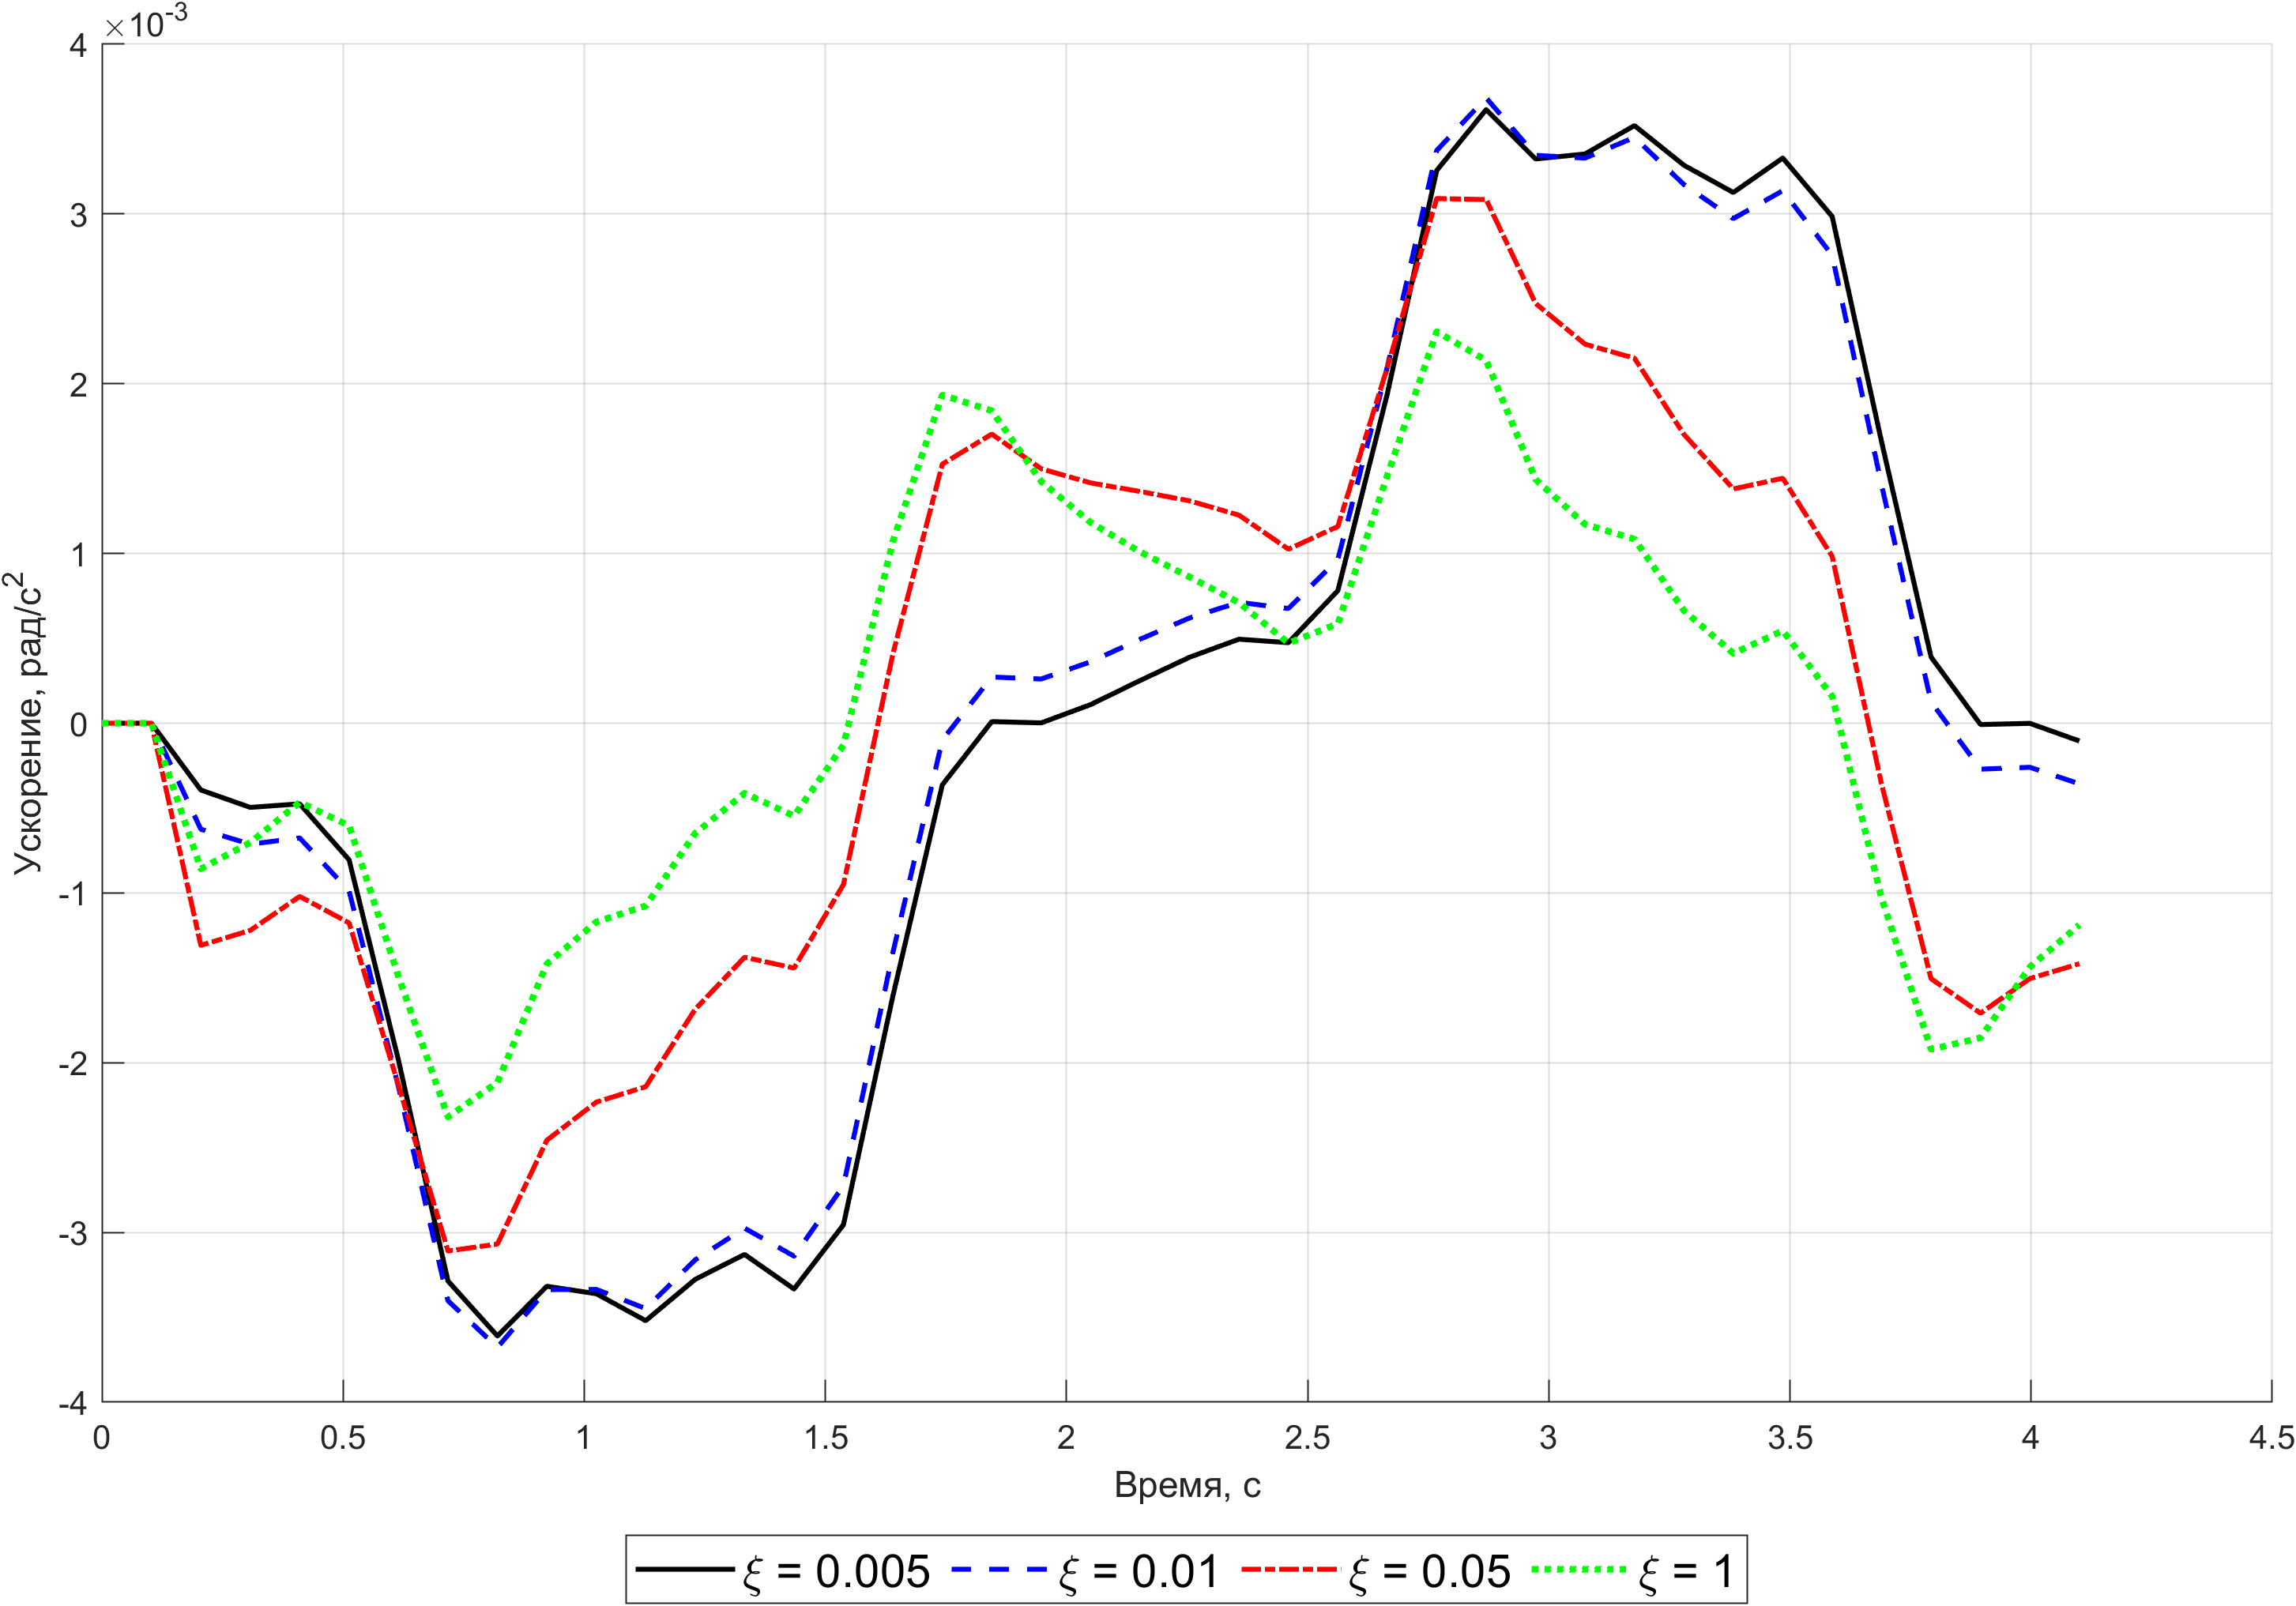
\includegraphics[scale=0.7]{matlab/decrement.png}
	\caption{Ускорение рамы с различными декрементами затухания}
	\label{fig:decrement}
\end{figure}

График, на рисунке~\cref{fig:test_moment} может служить основой для генерации задания контура управления по скорости вращения измерительного маховика.
\todo{Грфик}



\section{Конструкция стенда}\label{sec:ch4/sect2}

Стенд, показанный на рисунке~\cref{fig:yoim}, представляет собой подвешенный на тросе металлическом тросе куб, в который помещается исследуемая подвижная оптическая система. В качестве средств измерения используются датчик эталонного момента и ВОГ. Датчик эталонного момента состоит из моментного двигателя и маховик, суммарный момент инерции которых составляет \SI{2.68e-4}{\kilogram\metre\squared}.

\begin{figure}[ht]
	\centerfloat{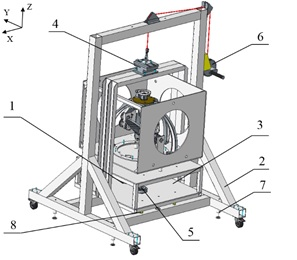
\includegraphics[scale=2]{yoiom}}
	\caption{Устройство относительного измерения остаточного момента}
	\legend{1 – маховик; 2 – платформа; 3 – измерительная платформа с изделиедержателем; 4 – зацеп настраиваемый; 5 – узел привода редукторного OZ; 6 – привод редукторный OZ;
		7 – волконно-оптический гироскоп; 8 – конус}
	\label{fig:yoim}
\end{figure}

Тестовое воздействие заключается в следующем. На двигатель-маховик подают управляющее напряжение, в результате чего он начинает вращаться по заранее заданному закону изменения угловой скорости. Угловые перемещения маховика измеряются преобразователем ЛИР-ДА190К. Крутящий момент от маховика передаётся на измерительную платформу с изделием-держателем, а скорость возникающих колебаний регистрируется волоконно-оптическим гироскопом.

В результате перемещения подвижной части изделия на основание стенда возникает крутящий момент, приводящий измерительную платформу с изделием-держателем в вынужденные колебания. Скорость этих колебаний фиксируется ВОГ.

Полученные показания подвергаются дифференцированию и последующей градуировке по эталонным значениям ускорения колебаний маховика, зарегистрированным при тестовом воздействии с заранее заданным кинетическим моментом.

В результате обработки данных определяется величина некомпенсированного крутящего момента, действующего на основание стенда при перемещении подвижной части ОМС. Пример полученных результатов измерений представлен на рисунке~\cref{fig:meauser_moment}.

\todo{график}

Абсолютная погрешность угломера ЛИР-ДА190К составляет
\[
\delta\varphi = 75''.
\]
При времени интегрирования
\[
t = 0{,}2\ \mathrm{с}
\]
это даёт погрешность угловой скорости
\[
\Delta\omega_m = \frac{\delta\varphi}{t}
= \frac{75''}{0,2\,\mathrm{s}}
= 0{,}1^\circ/\mathrm{s}
\approx 1{,}75\times10^{-3}\,\mathrm{c}^{-1}.
\]

Следовательно, относительная погрешность измерения угловой скорости маховика равна
\[
\delta_{\omega}
= \frac{\Delta \omega_m}{\omega_{\max}}
= \frac{1{,}75\times10^{-3}\,\mathrm{s}^{-1}}{18{,}65\,\mathrm{s}^{-1}}
\approx 9{,}38\times10^{-5}.
\]

% ------------------------------
% Погрешность измерения времени
% ------------------------------
Единица измерения времени \(\Delta t\) определяется числом тактовых импульсов контроллера за 1 с. При опорной частоте контроллера
\[
f_0 = 8000\ \mathrm{Гц}
\]
абсолютная погрешность измерения времени составляет
\[
\Delta t = \frac{1}{f_0} = 5\times10^{-4}\,\mathrm{s},
\]
что соответствует относительной погрешности не более
\[
\delta_t = \frac{\Delta t}{1\,\mathrm{s}} = 5\times10^{-4}.
\]

Эталонный момент на основание стенда от измерительного маховика $M_m=\SI{0,005}{Н\meter}$. Тогда требуемое значение ускорения $\frac{\Delta\omega_m}{\Delta t}$ измерительного маховика на линейном участке измерения скорости составит $\frac{\Delta\omega_m}{\Delta t} = \frac{M_m}{J_m}=\SI{18,65}{рад/c^2}$.

Таким образом основным источником погрешности при оценке остаточного момента на стенде является относительная погрешность гироскопа ВОГ ОИУС-1000 (0,01). Погрешность дискретизации времени $5 \cdot 10^{-4}$ по сравнению с этим пренебрежимо мала и увеличивает итоговую погрешность менее чем на 0,1 %.

Итоговая относительная погрешность измерений остаточного момента [16]

\begin{samepage}
	\begin{equation}
		\label{eq:final_moment_err}
		\begin{alignedat}{2}
			\delta M_m = \sqrt{(9,36 \cdot 10^{-5})^2+(1,9 \cdot 10^{-3})^2+(1\cdot 10^{-2})^2}
		\end{alignedat}
	\end{equation}
\end{samepage}

\section{Методика измерений}\label{sec:ch4/sect3}

Метод основан на сравнении неизвестного момента, возникающего при работе штатного двигателя изделия, с известным тестовым моментом, создаваемым тестовым маховиком на механической платформе стенда. Описание включает принцип действия, состав средств измерений, порядок проведения испытаний и обработку результатов, обеспечивающие воспроизводимость, обоснованность и требуемую точность измерений.

\subsection{Теоретическая основа методики}

При разгоне тестового маховика с моментом инерции $J_m$ и угловым ускорением $\varepsilon_m$ создается реактивный момент, согласно закону сохранения импульса:
\begin{samepage}
	\begin{equation}
		\label{eq:final_test_moment}
		\begin{alignedat}{2}
			M_m(t)=J_m\varepsilon_m(t)
		\end{alignedat}
	\end{equation}
\end{samepage}
Этот момент через подвесную раму передается на измерительную платформу, вызывая её угловые колебания.

Некомпенсированный момент штатного двигателя $M_{нк}$ вычисляется по отношению ускорения платформы:
\begin{enumerate}
	\item Измеряют угловое ускорение платформы $\varepsilon_{пл_m}$ при воздействии тестового момента $M_m$.
	\item Измеряют угловое ускорение платформы $\varepsilon_{пл}$ при повороте штатного двигателя оптической системы
\end{enumerate}

В приближении пренебрежения трением:
\begin{equation}
	\label{eq:Mnk}
	\frac{\varepsilon_{\text{пл}}(t)}{\varepsilon_{\text{пл,m}}(t)}
	= \frac{M_{\text{нк}}(t)}{M_m}
	\quad\Rightarrow\quad
	M_{\text{нк}}(t)
	= M_m,\frac{\varepsilon_{\text{пл}}(t)}{\varepsilon_{\text{пл,m}}(t)}
\end{equation}

С учетом трения $M_{тр}(t)$:

\begin{equation}	
	\label{eq:Mnk_trenie}
	M_{\text{нк}}(t) + M_{\text{тр}}(t)
	= M_m\frac{\varepsilon_{\text{пл}}(t)}{\varepsilon_{\text{пл,m}}(t)}
\end{equation}

Основные погрешности:
\begin{enumerate}
	\item Шум и дрейф гироскопа;
	\item погрешность датчика угла маховика;
	\item нелинейность и скорость-зависимое трение платформы;
\end{enumerate}

Оборудование, используемое в ходе измерений представлено в таблицах \todo{таблицы}

\begin{table}
	\centering
	\begin{threeparttable}
		\caption{Исходные данные}
		\label{tab:unit:measuring_equipment}
		\begin{tabular}{llc}
			\toprule
			Прибор                  & Модель              & Метрологические характеристики             \\
			\midrule
			Волоконно-оптический гироскоп       		& ОИУС-1000      				& Диапазон измерений угловой скорости $\pm550 \circ/с$        \\
			Преобразователь угловых перемещений         &ЛИР-ДА190К          			& Диапазон измерений $0^\circ \dots 360^\circ$ Пределы 			допускаемой абсолютной погрешности измерений $\pm10"$ \\
			Осциллограф            						& TDS1012В          			& Диапазон установки коэффициентов отклонения 10 мВ/дел - 5 В/дел. Погрешность установки коэффициентов отклонения $\pm3 \%$. Диапазон коэффициента развертки 5 нc      \\
			\bottomrule
		\end{tabular}
	\end{threeparttable}
\end{table}

\subsection{Калибровка приборов}

Важнейший этап подготовки экспериментального стенда --- калибровка волоконно-оптического гироскопа. Цель калибровки заключается в минимизации систематических ошибок, учёте температурных эффектов и оценке характеристик случайных флуктуаций. Процесс калибровки включает следующие основные этапы:

\subsubsection{Снятие нуля и оценка дрейфа}

Гироскоп устанавливают в неподвижное положение на виброизолированном стенде. Выходной сигнал~$\omega_g(t)$ снимают в течение двух часов с частотой $f_s = \SI{100}{\hertz}$
Результаты приведены на рисунке~\ref{fig:gyroEarth}.

\begin{figure}[ht]
	\centerfloat{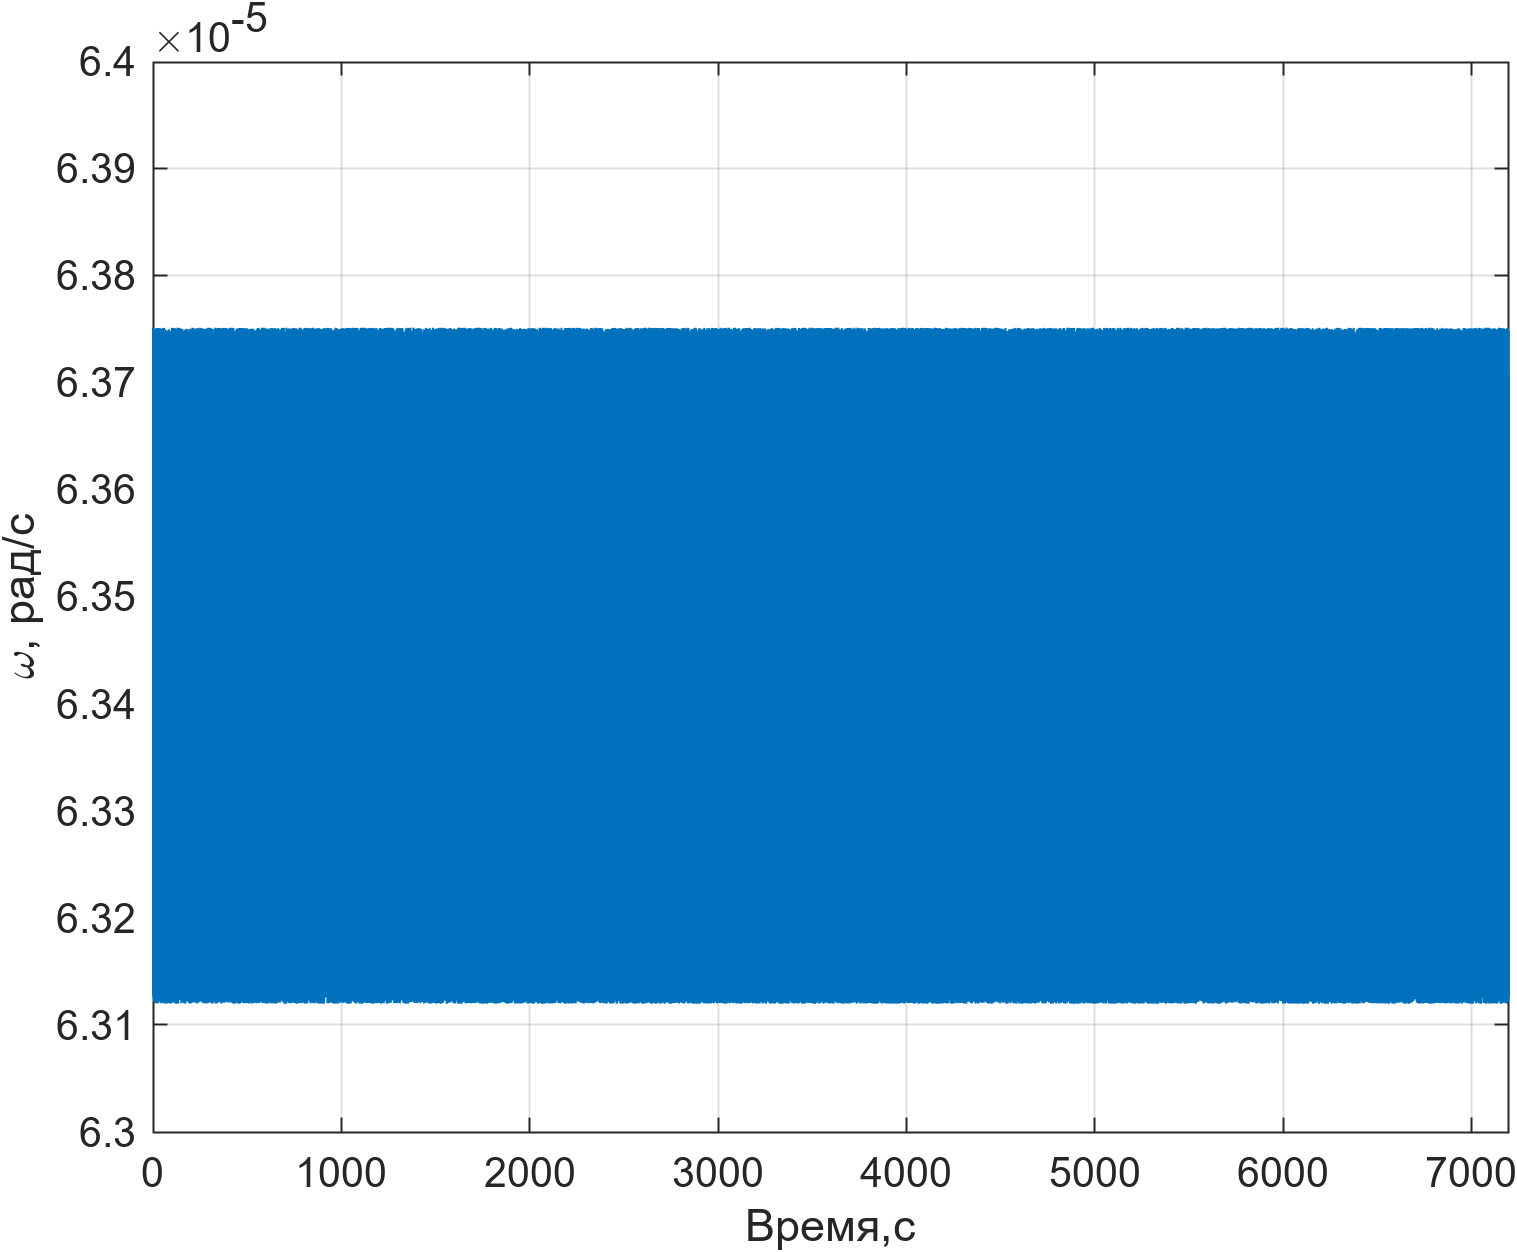
\includegraphics[scale=1]{matlab/gyroEarth.png}}
	\caption{Измерение проекции угловой скорости вращения Земли}
	\label{fig:gyroEarth}
\end{figure}

Математическое ожидание сигнала гироскопа:
\begin{equation}
	\bar{\omega}
	= \frac{1}{N}\sum_{i=1}^{N}\omega_g(t_i)
	\label{eq:mean}
\end{equation}

По расчетам среднее значение составляет 
$
\bar{\omega} = \SI{6,34 e-5}{\text{рад/c}}
$

Угловая скорость вращения Земли
$\Omega_E = 2\pi/T_{\text{сут}}\approx \SI{7,292 e-5}{\text{рад/с}}.
$
На широте города Санкт-Петербург $\phi_{\mathrm{e}} = 59^\circ57'$ получаем проекцию на вертикальную ось гироскопа:
\[
\omega_e
= \Omega_E\sin\phi_{\text{e}}
\approx 7.292\cdot10^{-5}\sin(59^\circ57')
\approx 6.32\times10^{-5}\text{рад/с}\\
\]

Скорректированное нулевое смещение:
\begin{equation}
	\bar{\omega}_0'
	= \bar{\omega} - \omega_e = \SI{3,16 e-7}{\text{рад/c}}
	\label{eq:omega_correct}
\end{equation}

Оценка шумовой составляющей. Дисперсия определяется по формуле:
\begin{equation}
	\sigma^2=\frac{1}{N-1}\sum_{i=1}^N(\omega_i-\bar{\omega})^2
	\label{eq:disperssion}
\end{equation}

Дисперсия составляет: $\sigma^2=\SI{3,15 e-7}{\text{рад/c}} \approx \SI{0,006}{^\circ /c}$

Коррекция температурного дрейфа.
Гироскоп помещают в термокамеру и проводят серию замеров в диапазоне температур от 15 °C до \SI{40}{\degreeCelsius} с шагом \SI{5}{\degreeCelsius}.

В каждом диапазоне вычисляем среднее смещение относительно нуля:

\begin{equation}
 	\bar{\omega}(T_j)=frac{1}{N} \sum_{i=1}^N\omega_i(T_j)
 	\label{eq:omega_mean_T}
\end{equation}
 
 
Стандартное отклонение дрейфа:
\begin{equation}
	\sigma_{\mathrm{др}}
	= \sqrt{\frac{1}{N-1}\sum_{i=1}^{N}\bigl[\omega_{\mathrm{др}}(t_i)\bigr]^2}\,.
	\label{eq:sigma}
\end{equation}

Переход к угловому ускорению
Численно дифференцируют исходный сигнал и температуру центральной разностью

Поскольку в дифференцировании константы $\bar{\omega}_0'$ и $\omega_e$ исчезают - окончательная формула для углового ускорения:





\subsection{Алгоритм измерения}

 
 
 
 





